\documentclass[aspectratio=169]{beamer}
\usetheme{metropolis}
\usepackage{amsmath}
\usepackage{amssymb}
\usepackage{braket}
\usepackage[sorting=none, maxnames=1]{biblatex}
\addbibresource{main.bib}

\usepackage{xpatch}

\xpatchcmd{\itemize}
  {\def\makelabel}
  {\ifnum\@itemdepth=1\relax
     \setlength\itemsep{1ex}% separation for first level
   \else
     \ifnum\@itemdepth=2\relax
       \setlength\itemsep{0.5ex}% separation for second level
     \else
       \ifnum\@itemdepth=3\relax
         \setlength\itemsep{0.5ex}% separation for third level
   \fi\fi\fi\def\makelabel
  }
 {}
 {}

\metroset{block=fill}

\definecolor{success}{RGB}{121, 174, 144}
\definecolor{fire}{RGB}{216, 65, 65}
\definecolor{aqua}{RGB}{16, 34, 64}
\definecolor{sand}{RGB}{241, 237, 229}
\colorlet{xsand}{sand!50}
\setbeamercolor{normal text}{fg=aqua, bg=xsand}
\setbeamercolor{alerted text}{fg=success}

\author{David Bucher}
\title{Incorporating Inequality Constraints into QAOA}

\begin{document}

\maketitle

\section{QAOA Brief Introduction}


\begin{frame}{The Quantum Approximate Optimization Ansatz}
\begin{center}
    \begin{itemize}
        \item Variational circuit for combinatorial optimization, introduced
            by~\citeauthor{farhi2014}~\cite{farhi2014}
        \item Trotterization of quantum annealing: $\hat H(t) = (1-t) \hat H_M +
            t \hat H_P$
        \item Problem Hamiltonian $\hat H_P = -\sum_{i,j} J_{ij} \hat \sigma^z_i
            \hat \sigma_j^z - \sum_i h_i \hat \sigma_i^z$
        \item Mixer $\hat H_M = -\sum_{i} \hat\sigma^x_i$, Initial state $\ket{+} = -\hat H_M \ket{+}$
    \end{itemize}
    \vspace{6pt}
    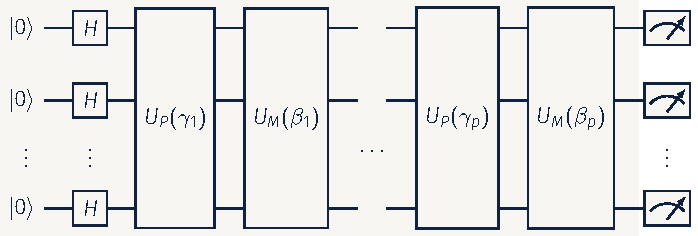
\includegraphics[height=3.0cm]{graphics/build/qaoa.pdf}
\end{center}
\end{frame}

\begin{frame}{The Quantum Alternating Operator Ansatz}
    \begin{itemize}
        \item Generalization of the ansatz by~\citeauthor{hadfield2019}~\cite{hadfield2019}
        \begin{itemize}
            \item $U_P(\gamma)$ \emph{phase-separating} unitary that depends on
                \emph{objective function}
            \item $U_M(\beta)$ \emph{mixing} unitary that depends on
                \emph{domain}
        \end{itemize}
    \end{itemize}
        \begin{block}{Condition for Mixer}
            Map between all feasible states
        \[
            \forall \mathbf{x}, \mathbf{y} \in F,  \exists \beta :
            |\bra{\mathbf{x}}
            U_M(\beta)  \ket{\mathbf{y}}| > 0
        \]
        \end{block}
\end{frame}

\section{Inequality Constraints Before}


\section{Constrained Mixer for Inequality Constraints}


\section{Experiments}

\begin{frame}[allowframebreaks]
    \frametitle{References}
    \printbibliography[heading=none]
\end{frame}

\end{document}
